% This example An LaTeX document showing how to use the l3proj class to
% write your report. Use pdflatex and bibtex to process the file, creating 
% a PDF file as output (there is no need to use dvips when using pdflatex).

% Modified 

\documentclass{l3proj}
\usepackage{float}
\usepackage{caption}
\usepackage{subcaption}
\usepackage{url}

\usepackage{csquotes}

\begin{document}

\title{Team CS04 - TrypAdvisor}

\author{Amy Kidd -- 2295291K\\
        Elizabeth Boswell -- 2398840B\\
        Inesh Bose -- 2504266B\\
        Jingqi Li -- 2431138L\\
        Mihhail Pikkov -- 2406150P}

\date{April 2021}

\maketitle

\begin{abstract}
\normalsize In the field of medical statistics, technology has been shown to be the fastest and most efficient way of globally collecting data. For example, in the COVID-19 outbreak many different apps were released by government groups to track and monitor outbreaks around the country.

This paper is a reflective piece analysing the process of creating software for the Institute of Biodiversity, Animal Health and Comparative Medicine, which is to be used in the monitoring and surveillance of sleeping sickness. It will go on to study the team's management practice and agile processes incorporated throughout this project to deliver the set requirements, as well as discuss challenges the team faced, and draw conclusions on the lessons learned over the last six months.
\end{abstract}

%% Comment out this line if you do not wish to give consent for your
%% work to be distributed in electronic format.
\educationalconsent

%==============================================================================

\newpage

%==============================================================================
\section{Introduction}
This paper presents a case study of the development of TrypAdvisor, a web application used to submit records and track data for African trypanosomiasis, otherwise known as sleeping sickness. It is to be used by members of the public, health care workers and researchers, mainly in Africa.

The report starts by discussing the \hyperref[sec:background]{project background}, describing the customer and project objectives as well the state of the final product. Afterwards the report will have a \hyperref[sec:reflection]{reflection} on the software practices used over each \hyperref[subsec:iterations]{iteration}, and will discuss any issues that have arose during the project. In the section the \hyperref[subsec:practices]{software practices} will be analysed and how successful the team felt the methods used were. This will then lead into an analysis of the \hyperref[subsec:iterations]{iteration} methods, in particular the adaptive software development model that the team used. The report will also dive deeper into the design decisions that were made by the team, and the \hyperref[subsec:qa]{quality assurance} measures taken in development and study the issues in development. There will be a special focus on the issues encountered during the realisation of three of the project's main objectives - \hyperref[subsec:us]{usability}, \hyperref[subsec:datacol]{data collection} and \hyperref[subsec:datarev]{data review}. Here, the report finds that the main causes of problems were insufficient research into the technologies used, conflicting requirements, and requirements that were not specific enough to the target audience. In the final section, \hyperref[sec:conclusion]{conclusion}, there will be a discussion of the overall take away of the application and the wider lessons the team has learned about the processes of software engineering in relation to the agile methods used in many other development practices. 

%==============================================================================
\section{Case Study Background}
\label{sec:background}

\subsection{Customer and Background}
The Institute of Biodiversity, Animal Health and Comparative Medicine is a research institute of the University of Glasgow which studies \textquote{a spectrum of areas from veterinary science through to fundamental research in ecology and evolution}\cite{BAHCM}. The team's point of contact was research associate Dr. Walt Adamson, who specialises in the field of virology, in particular parasitic transmission from animals to human. He works with a number of people within the UK and Africa to monitor sleeping sickness outbreaks, and the goal of the project was to develop an app that makes the monitoring more effective. Even though the team's customer had little understanding of the process of building software he was extremely engaged throughout the development and had a clear view of the features he wanted, whilst also being open to new ideas.

During the initial meeting, goals were quickly outlined and expectations managed. The team's first agreement was switching from a mobile app, which the customer had previously wanted, to a web application. The team decided that this better fit the needs of the users, who might have old devices with little storage space and would be reluctant to download another app just to fill out a survey. Having the application online also meant that future changes can be more easily implemented without the need for software updates on users' phones. Another advantage of a web app is that it is equally accessible from non-mobile devices.

In the first couple of iterations meetings with the client were set up on a weekly basis, and communication was held over a Microsoft Teams channel. The communication was punctual and effective, adhering to the regularly scheduled meetings. Considering the customer's lack of technical knowledge, it was expected to be a challenge filling the customer in on the developed features. The team had to keep this in mind when explaining technical aspects of the project. To ensure that the final product met the expectations, the team often relied on existing examples of web applications when discussing desired features to be implemented. This way the customer could describe his needs without the technical terms or experience. As the project progressed, the team moved on to mainly use the customer days to demonstrate and review newly implemented features, whilst still staying in close contact over the Microsoft Teams channel. This was due to the group's increasing knowledge and understanding of the project, which decreased the need for structured guidance on the wants of the customer. Early on in the development process, the customer was also given the link to the hosted web application for review for himself and his colleagues.

\subsection{Project Objectives}
In the initial stage, using the customer's briefing, the team identified the rationale and objectives for the project and came up with a general set of fundamental goals that the web application should meet.
\begin{itemize}
    \item \textbf{Usability} - The web application should include minimal textual input and instead present the user with buttons, and should make use of images and colours. This is because there could be different levels of literacy and potential language barriers among users, so the costumer wanted the application to convey questions in the simplest form. As the website might be used on low technology devices, it was decided to keep the UI design minimal while also creating an enjoyable experience. This is similar to other software like Scotland's COVID-19 tracking app Test and Protect \cite{TestandProtectScotlandApp} and C19byZoe \cite{C19byZoe}. They both use bright and simple designs to monitor COVID data. 
    
    \item \textbf{Data Collection} - This should be done through the submission of forms. Three different types of users were identified: members of the public, health care workers and entomologists/veterinarians, each of which would have their own separate form with questions specific to their expertise. 
    
    \item \textbf{Data Review: Table and Mapping} - The team understood that the viewing of the gathered data was just as important as the collection. The customer expressed an interest in having a map with a geographical representation of the data as well as a table. Being able to export data in a spreadsheet format (CSV) was also important. The team took inspiration from maps provided by The Institute of Health Metrics and Evaluation \cite{IHME} which provide detailed visualisations of outbreaks of COVID-19 and other diseases.
    
    \item \textbf{Data Protection} - Since the team was dealing with sensitive medical data, security was a top priority. After a discussion with the client the team decided that it would be best to have an account system with the client as an administrator to monitor who is allowed access to this data. Anyone would be able to make an account, but the administrator would have to authorise an account to view the data. Towards the end of the development the team obtained a CA certificate for the application, enabling secure data transfer.
\end{itemize}

\subsection{Final Delivered Software}
The final product \cite{TryAdvisor} is a web application hosted on PythonAnywhere \cite{PythonAnywhere}. It was developed using Django \cite{Django} (Python) with Plotly \cite{Plotly}, an interactive graphing library that offers mapping functionalities. A user can submit medical data of sleeping sickness symptoms through a form, as seen in \ref{appendix:main}. The data can be viewed by logged in and verified users in a table and on a map. Admin users, such as the customer, can edit the questions on the form as well as change the location data and officiate registered users to view the table and map. Non-registered users can access a form for members of the public, while registered users can also access forms meant for healthcare workers and entomologists/vets.

The table shows the location of a person that filled out a form, and the answers that they gave. The location is gathered through the browser's GPS functionality, manual entry of the location, and conversion of the entered location into coordinates through the geocoding service Nominatim \cite{Nominatim}.

The map page features a world map and a map of Africa. Markers on the map show the location of persons that filled out the form. The colour of the markers indicate through which method the coordinates were obtained. Hovering over a marker displays a popup box, which initially only shows the exact coordinates and how they were obtained. A dropdown menu with all symptoms and questions makes it possible to refine the selection of data and show the responses given. Both the map page and the table page include the option to export the data as a CSV file. The concepts of these features can be seen in appendix \ref{appendix:wireframes}.
%==============================================================================
\section{Reflection}
\label{sec:reflection}

\subsection{General Software Engineering Practices}
\label{subsec:practices}
The project's development process was done through the agile development methodology which, as the name would suggest, is about moving a feature from backlog to delivered in the quickest and easiest way possible. Whilst researching into this method of practice, it was noted from a variety of different studies that agile was the most successful software development process. Agile modelling showed 72\% of agile projects were deemed successful compared to more traditional methods and the overwhelming majority of people rating it `much higher' in terms of team productivity, quality and stakeholder satisfaction compared to other approaches \cite{AgileSuccess}.

As part of the agile framework and at the request of the university coordinators, the team practiced scrum management which defined the team members into different roles to aid the development process. Roles coordinated during the initial project setup were scrum master, who leads and trains the team and monitors the progression of the project, a product owner, who takes ownership of a feature and is responsible for communication of updates on that topic with the client, and finally the developers, who take accountability of issues to deliver in increments.  

As part of Scrum, every week the team conducted a stand up meeting coordinated by the scrum master. According to the Scrum Guide \cite{ScrumGuide}, \textquote{Daily Scrums improve communications, eliminate other meetings, identify impediments to development for removal, highlight and promote quick decision-making, and improve the Development Team's level of knowledge. This is a key inspect and adapt meeting} \cite{DailyScrum}. During the meetings each team member would discuss what they had done over that weekly period, what they are working on for today, their planned achievements and if there is anything blocking them from doing this. These meetings were kept short, to around 15 minutes and as a rule the actual code itself could not be spoken about in detail, if needed a later planning meeting or code review could be scheduled.

Although scrum was a suggested practice from the project's supervisors in comparison to its competitor method, Kanban, the team felt like scrum was a better fit of practice because of these defined roles that the team had. This allowed the team to have better structure and accountability throughout the project. Scrum also places a heavier emphasis on iterative methods such as daily stand ups compared to the lack of time boxing in Kanban \cite{ScrumvsKanban}. As a team new to the software engineering practice, the team members found this aspect extremely beneficial to use, as some felt more comfortable taking notes and writing down main talking points, while another could interact freely with the customer without any interruptions. Overall, working in a scrum driven agile development team helped drive the productivity and keep everyone accountable of the specific tasks from the structure methods specifically defined in scrum as compared to Kanban methodology.


\subsection{Iterations}
\label{subsec:iterations}
After researching and comparing different models of software development life cycles \cite{SDLC}, the team chose the adaptive software development (ASD) model to make sure the team was meeting its targets. This was due to its the quick and evolving work flow with Scrum board style tracking. The team used a similar method to what is discussed in the Agile Review and Analysis e-book \cite{IterationReviewAndAnalysis}. It explores adaptive development cycles as a form of iteration method by dividing the cycle into 3 main components: \hyperref[speculate]{speculate}, \hyperref[collab]{collaborate} and \hyperref[learn]{learn}. 

\subsubsection{Speculate}
\label{speculate}
The team's speculation period usually took place at the start of every month after the team received a large backlog of issues from the previous client day, and consisted of using a mixture of user stories and MOSCOW \cite{MOSCOW} methods for bigger features as defined in \hyperref[sec:background]{project objectives}. Team members first identified the types of users who would have access to a feature from the set of user personas \ref{appendix:UPandS}. Then, the team members thought of the functionality that this feature must have, should have, could have and would like to have. Using this technique the team could then develop issues from the discussed points. 

For example, when implementing the account system the team made use of this method to specify which privileges to give to each type of user. Some features, such as preventing entomologists and vets from accessing the form for healthcare workers, were not implemented, as the team decided this was a `would like to have' feature, and not essential to the functioning of the application. The reasoning was that a professional such as an entomologist would have little reason to pretend to be a healthcare worker. This allowed the team to focus its attention on the `must have' features, which were to only allow professionals to fill out forms for professionals, and to only allow authorised professionals to access the collected data.


\subsubsection{Collaborate}
\label{collab}
During the collaboration process the team worked on developing the features of the project, which were to be presented at the end of the month to the customer. Each code change, apart from small and urgent bug fixes, was introduced through feature branches and merge requests. A team member would pick an issue to work on, develop the functionality on a feature branch and then create a merge request.

During this time, a number of different collaboration techniques were used to aid the learning and understanding of the team. A main source of collaboration within the team were code reviews. After submitting a merge request, someone reviewed the code and, if necessary, extended the functionality. The reviewer used Microsoft Teams to ask for clarification and point out problems with the code. Once the code was in a satisfactory state it was merged into the master branch. Using code reviews is not only an effective way to keep other members informed about how the code is developing, but also a way to reduce the number of bugs, as two people can notice more than one \cite{Inspections}. These code reviews were used throughout the duration of this project, with over 50 merge requests approved by a different member on the team from the person who wrote the code.

When using feature branches it is essential to ensure that a feature branch is merged with the newest version of master before merging it into the master branch. This practice took some time getting used to, and occasionally changes in the master branch were overridden by a merge because the branch was not merged with master properly. The code reviews helped with this to some extent, but reviewers would sometimes also forget to ensure that the branch is up to date. The process might have also been made more difficult by the fact that the team worked from several different countries and time zones - a lot of work was done asynchronously and it was easy to miss something that someone else had changed. The issue was eventually solved by improving team communication, discussing the problem in retrospectives and stand up meetings, and simply getting used to the practice.

Another collaboration method the team tried was pair programming. This was led by someone working on a bigger feature with another less knowledgeable person to work together so it could then be eventually branched off individually. Pair programming was also used in areas where both participants had little understanding of a new feature as ideas could be better discussed together. However due to time differences and virtual communication pair programming took a large amount of planning and coordination, so code reviews where used in favor of this as they could be done at any time with a short follow up meeting if necessary. While Böckeler and Siesegger \cite{codeReviewsPairProg} argue that code reviews are no substitute for pair programming because they don't require the same amount of cooperation and cause disruptions to the usual workflow, the team did not find this to be the case. In fact, the more asynchronous nature of code reviews was an advantage, and was less disruptive than having to plan a pair programming session. Code reviews also offered sufficient opportunities for discussion and collaboration.

\subsubsection{Learn}
\label{learn}
The full or partial completion of the team's goals for the iteration led to the final part of the ASD process; the learning stage. The team used the customer meetings to gain feedback and gauge the customer's satisfaction through a demonstration of the updated application. This was used to review the current code and to create new features and user stories, which would then be sectioned into individual issues. Before the customer day an agenda was made, and each person was assigned a role. The roles used were the meeting chair, who hosted the meeting and slides, project owners who demonstrated the features they were working on, and a note taker. The agenda included time slices for every topic, to make sure that there was time to discuss key points and to answer questions. 

Another part of the team's learning stage involved analysing the team's communication and working through the use of retrospectives. They were used to gain knowledge about how everyone was feeling, and to provide a safe and honest place to outline any blockers. The team used an application called GoRetro \cite{GoRetro} to conduct the retrospectives, as it was easy to use virtually. The categories `what went well' (liked), `what didn't go well' (learned) and `what can be improved' (lacked) were used to reflect on important occurrences in the previous iteration. The team then tried to identify possible improvements, leading to increased productivity and communication within the team. For example, in the first retrospective the team found that some team meetings had low attendance. A root cause analysis showed that this was because some members did not get notifications for all posts on the Microsoft Teams channel, and thus were not reminded of the meeting. Everyone was encouraged to turn on all notifications, and the scrum master started sending out more invites. These steps increased awareness of meetings, and thus led to higher attendance.

\subsection{Quality Assurance}
\label{subsec:qa}
As the work in progress was accessible to the customer for review it was necessary to maintain a high standard of code reliability and clarity. To maintain a homogeneous code structure the code was periodically linted using \texttt{black} \cite{black}. This made it easier for team members to extend other people's code, as they did not need to first get used to individual programming styles.

A unit test suite was developed alongside the product, the goal was to add a unit test after the implementation of each new piece of functionality that could feasibly be tested \cite{UnitTest}. This was not always done, tests were often added in bulk after the fact. The team decided not to adopt a test-driven development approach because none of the members were familiar with the practice, so it seemed too difficult and risky. In spite of all this the test suite proved to be very effective, with a test code coverage of 79\% at the end of the project. It was also useful in practice. For example, the team used the \texttt{django\_tables2} module to render the table on the table page, before switching to a custom solution towards the end of the project. This module was slightly difficult to work with, especially because it was not well-suited to the database layout. Having a set of tests for the tables page prevented many defects from accidentally being introduced into this page.

Periodic mutation testing, using \texttt{django-mutpy}, showed mutation scores of around 93.0\%. Mutation testing was not introduced into the CI/CD pipeline because it takes too long - at the end of the project running \texttt{django-mutpy} took around two minutes. However, it would have been been beneficial to do mutation testing during the ASD `learn' phase. This would have given the team an idea of the current quality of the test suite and how it could be improved. Similarly, the test code coverage was only calculated from time to time. These efforts were probably not taken because the main focus was to develop the features that the customer wanted. Testing was a less visible and time-critical activity, and considering that implementation of a test sometimes took the same amount of time as the feature's development process, it was talked about less often \cite{Testing} and took less of a priority.

The repository was set up with a three stage job CI/CD pipeline. The first job would run the unit tests for the application. Then, the second would deploy the application on the development and testing server. Finally, the third job would deploy it on the production server. This would prevent the customer from experiencing any issues with the app as it was developing. 
The deployment was done on Heroku with the help of Dpl \cite{gitlabdpl}. However, it was realised that the pipeline ran very frequently after continuous commits and took too long, therefore the jobs were made more time and event specific. The tests would only run on merge requests (since new features are introduced through merge requests) and deployment to the development server would only occur on the \texttt{master} branch (e.g. after a merge request). Periodically the \texttt{master} branch would be merged / made `even' with the \texttt{deploy} branch that would deploy the application on the production server. This way, the pipeline was essentially broken down into three scenarios where only one job would run.

To make the application easier to set up, all dependencies were continuously reviewed and questioned to avoid any version mismatch or compatibility issues.
As mentioned above, one of the dependencies that the project got rid of was \texttt{django\_tables2} because it was not well-suited to the database structure and did not include any special features like being able to rename column headers. The dependency was removed after the application enabled exporting the data into a CSV format, since the process of rendering the table is similar. 

The project was decided to be open-source from the beginning and therefore needed a suitable license. This was factored by the intended usage of the application. After reviewing the licensing of the 39 (direct and indirect) dependencies and with the help of Choose A License \cite{ChooseALicense}, the team went with the MIT License \cite{MITL} without much doubt. It is simple and to the point. While GNU General Public License \cite{GNUGPL} v2.0 and v3.0 were considered, it is conditioned to be used with the same license which does not give flexibility to users. Fortunately, none of the dependencies had the GNU GPL license (most were MIT and BSD-3 \cite{BSDL}).

\subsection{Usability Development}
\label{subsec:us}

Since the web app was meant to be used on mobile devices, the visual interface had to be made responsive by automatically shifting, resizing or hiding some UI elements. For example on mobile the top navigation panel is hidden in a menu button to reduce screen clutter and enable easier navigation. However, it was not straightforward to implement responsive design for the table and the map pages, as they cannot be resized arbitrarily. The decision was made not to pursue the responsive design of those two particular pages, as the researchers are more likely to access them on a computer. Another feature that was dropped was a progress bar which would represent how many questions the user has answered. This was difficult to implement due to the structure of the database and the ability to skip questions. The team decided not to implement it as issue prioritisation showed that it was a `nice to have' feature.

For the symptom questions the team used publicly available stock images to visualise medical conditions like a fever or rash. The team quickly noticed the lack of available photos depicting people of African ethnicity. The customer agreed to research this matter and provide the team with appropriate images, while in the meantime the team resorted to using the images with people of white complexion. In addition to this, the customer agreed to provide the team with images specific to sleeping sickness, like a picture of a trypanosomal chancre. However, possibly due to lack of resources, the customer was unable to provide the team with necessary images, and the images remained unchanged. However, the team provided the customer with a way to address this issue in the future by using the administrative capabilities of the application to change the question images manually.

The web app is meant to be used in several African countries, and by speakers of many different languages. Being able to display the site in these languages is essential to allow a large number of people to use the web app, especially because some of these languages are not available on Google Translate or similar services. From the beginning the team ensured that the names of symptoms and the associated questions would be translatable. This was done by representing symptoms as database items that could be edited by admin users. However, the question of translating the rest of the application only arose during the last iteration. Towards the end of the development the templates were changed to support manual translation via \texttt{gettext}, which, in principle, yielded a fully translatable application. 

However, it is necessary to maintain different databases for different languages, as there is no way to differentiate between symptoms of different languages in the database. This means that different language implementations need to be hosted on different websites. It would have been better to allow the database to support multiple languages, for example by adding a language field to each symptom. This would make it possible to host all language implementations on the same site, and to toggle between languages. This issue would not have come up if full translation had been seen as a `must have' feature, which might have been the case if requirements had been gathered more carefully, and if user stories had been adapted to reflect the language needs of the target audience.

To summarise, the main challenge in reaching the usability goals was adapting the application to the specific needs of the users. Overall, usability has been achieved to a good standard, though some minor features had to be dropped due to a lack of time and resources. In the case of translation, more thorough requirements gathering could have led to a more flexible and appropriate solution.

\subsection{Data Collection Development}
\label{subsec:datacol}
The team's \texttt{models.py} does not follow the `fat models and thin controllers' pattern \cite{BestPractices}. Models either have no methods or only have standard methods such as \texttt{\_\_str\_\_()} and \texttt{save()}. This was because the team was under the impression that the models should be simple objects that represent database items, and all the business logic should be in the views. As a result, some of the views are quite complex in order to enable the models to be as simple as possible.  It is hard to say how much using `fatter' models might have improved the quality of \texttt{views.py}, as the team did not become aware of this convention until after the code freeze, and has not done much research on this topic beforehand. Still, it would have been beneficial if the team had made itself familiar with Django's best practices before starting the project.

Initially, the team wanted to keep open the possibility of the application being turned into a mobile app as well. However, this would require using different frameworks for the mobile app and the web app, and so there may be different database instances for each platform, similar to how a Django project has one default instance of the \texttt{db.sqlite3} file. A solution to this was to use MongoDB and its cloud database. This database could then easily be connected to the applications using Atlas. All it required was the connection string and data would be parsed as JSON. For Django, a package called `\texttt{djongo}' was used to realise this.

However, this was not necessarily considered `good practice' during development and testing and it was creating issues - all instances of the application, including the production server, were connected to the same database, so all migrations (including test migrations) were being reflected on all instances.

Apart from these development issues Django did not work as desired in terms of reliability (raised \texttt{DatabaseError} at random times) and performance with the database, mainly because MongoDB uses NoSQL (JSON) format queries, but Django relies on SQL. Therefore, the database was changed back to SQLite (the Django default). But to solve the initial goal of having a consistent, unified and accessible database (instance), a REST API was developed using the Django REST Framework \cite{DRF}. This meant the data could be added and fetched using POST and GET requests from all possible applications related to this project.

In data collection, the main issue was a lack of knowledge of best practices and appropriate technologies. The team made design choices that seemed to make sense based on intuition and previous experience, but that did not correspond to Django best practices. In the case of the database implementation, the problem was successfully resolved once it was discovered. The problems caused by the `fat models and skinny controllers' were more subtle, and were noticed too late. They would not have occurred if the team had researched Django best practices beforehand.


\subsection{Data Review Development}
\label{subsec:datarev}
The ability to gather the user's GPS location through the browser was implemented fairly early (iteration 3) but it only ever worked locally, not on the deployed Heroku website. It was not until iteration 6 that the team discovered that this was because the deployed website did not have a CA certificate and was thus accessed through an HTTP connection, not an HTTPS connection. Unfortunately it is not possible to obtain a free CA certificate for a website hosted using Heroku's free plan, and the customer stated that he would prefer not to pay for the hosting. After some in-depth research into alternative hosting providers the team settled on using PythonAnywhere to host the website, as they offer a CA certificate with their free account. 

Hosting the website on PythonAnywhere presented a new challenge, however, as they do not allow access to private GitLab instances through their console. As a result the project was copied to a GitHub repository, which was kept private until a few days before the handover. This meant that the team did not use their CI/CD pipeline to deploy to PythonAnywhere. Instead, the team decided to keep the two Heroku instances up for the time being, and to periodically copy the application to GitHub as well. It would have been possible to set up a GitHub mirror repository, but the team was not aware of this possibility until after the customer handover. Perhaps asking for advice on how to handle this setup would have made it possible to use this functionality earlier in the development.

There are two things that the team can take away from this issue: the first is that it should have tried to identify the cause of the problems with the GPS feature early, instead of assuming that it would be easy to fix later. The second is that it is not always possible to find a solution that satisfies all requirements: the team could not find a web-hosting provider that was free, offered CA certificates, and worked with the team's current GitLab's CI/CD setup.

An unusual design decision is the choice to store location data as two sets of coordinates and a string. The initial plan was to only gather location information through the browser's in-built geolocation feature. A textbox for manual entry of the location should serve as a backup in case the user does not give the site location permission. A geocoding service would obtain the coordinates of that entered location, and they would be stored instead. The team chose the geocoding service Nominatim, as it is free, simple to use, and based on the relatively large Open Street Maps data set.

However, the customer soon informed the team that the geocoding service was often not able to obtain the coordinates of places. This is because African place names tend to have many different spellings or refer to multiple locations. An obvious solution would be to use a different geocoding service, but the team was not able to find a free service that was well-suited for African place names. Instead the team chose to store every location entry in plain text, alongside the GPS coordinates and the geocoded coordinates, if available. If any of these coordinates are incorrect or missing an admin user can change them through the admin interface.

Storing three kinds of location data in the database created some redundancy, which might have been eliminated by using a more powerful geocoder like the Google Maps API (a paid service). However, it ended up being a solution that the customer was satisfied with, as it allowed a lot of flexibility in the gathering and interpretation of location data. If the team had been able to find a better geocoder it might have been necessary to store the redundant information anyway, as it is not guaranteed that it will be able to recognise every single place name.
This experience showed the team that sometimes custom solutions are better than using more advanced technology, and that the nature of an ideal solution varies a lot between different projects.
The team's particular experience with geocoding African place names is not uncommon, as a 2018 paper by Kuhn and von Borzyskowski \cite{africaGeocode}, comparing the accuracy of manual and machine geocoding for sub-Saharan Africa, finds that \textquote{(...) human coding outperforms machine coding in sub-Saharan Africa to date in terms of both quality and precision}.

The challenging part of implementing data review was the collection of the location data. The solution had to be free, powerful, and suitable to African locations. It turned out to be very difficult to meet all these requirements simultaneously. Nevertheless, the team was able to find a compromise and implement custom solutions that fulfilled the requirements set to the best of their abilities. Some issues arose because the team delayed solving the CA certificate problem, and did not think of using a mirror repository. This could have been avoided by better issue prioritisation and more thorough research.

%------------------------------------------------------------------------------
\section{Conclusions}
\label{sec:conclusion}

TrypAdvisor was the team's first agile long-term software project and it provided a great practical experience for the team. While working on the project, the team has encountered some issues but also transferred these issues into lessons and improvements.

During the software development process, the team split up roles and workload using the scrum methodology with agile management. Iterations were managed using the adaptive software development model. This was to improve the team's efficiency, communication, and performance. However, in the early stages of the project, the team encountered some small problems with its organization and collaboration. One of the problems was low attendance in team meetings, which hindered the communication of the team. Thanks to the agile process, the team found a solution to this problem in the following retrospective and started adding more notifications for these meetings. By solving problems using agile methods, the team significantly improved their agile management skills.

One of the big technical and organizational issues was deciding which technology to use. This issue became the most apparent when deciding on the database implementation and deployment platform. Although these problems didn't bring a massive amount of trouble, they still had a negative effect on the team's efficiency and energy. These issues were caused by a lack of research into the target technologies. A better understanding of these technologies would have allowed the team to make a more cautious and appropriate decision.

Other issues were caused by requirements that were difficult to meet or that were not specific enough to the target audience. These include the problems faced when gathering location data or when implementing translation. The team was able to compromise and meet these requirements to a good or satisfactory extent, but in some cases, requirements could have been gathered more carefully.

During the project, the team members explored various technologies and gained new expertise in Django, Git, SQL, Bootstrap, Plotly and others. Some of them were not familiar to team members at all, which made the process more arduous. However, through this the team increased its ability to learn new things through research and self-study. This is a valuable skill that will be used frequently in the future.

In quality assurance, the team mainly focused on unit testing. Although the team did not follow test-driven development due to unfamiliarity, the test code coverage is still very high. This ensures that the code is of high quality, and will make future code changes easier. The team also benefited from the unit tests during the developing process as they increased the team's efficiency. In addition, it helped the team increase their quality assurance knowledge.

Overall, the team members improved many aspects of their software development skills through this project, and this experience will definitely provide a memorable and positive impact on their future projects and careers.

%==============================================================================
\bibliographystyle{plain}
\bibliography{dissertation}


%==============================================================================
\newpage

\section{Appendix}
\label{appendix}
\appendix

\section{Main page of the final product}
\label{appendix:main}

\begin{figure}[H]
  \centering
    \fbox{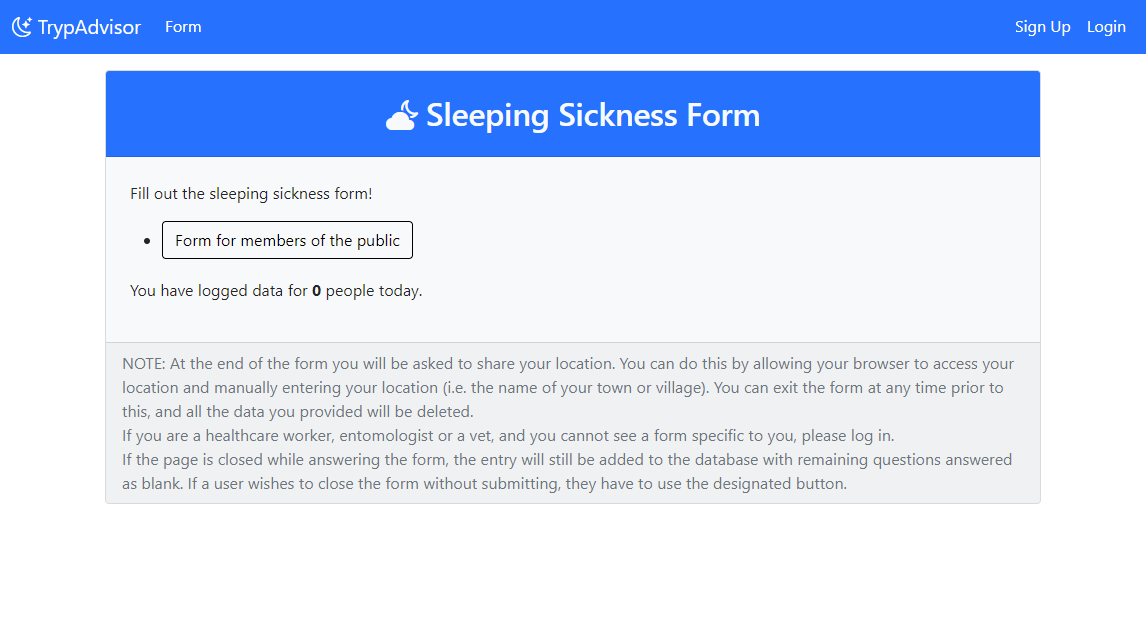
\includegraphics[width=0.7\textwidth]{images/FinalHome.png}}
  \caption{Final Delivered Software - Home Page}
  \label{fig:Final Home Page}
\end{figure}


\section{Wireframes}
\label{appendix:wireframes}

\begin{figure}[H]
\centering
\begin{minipage}{.5\textwidth}
  \centering
  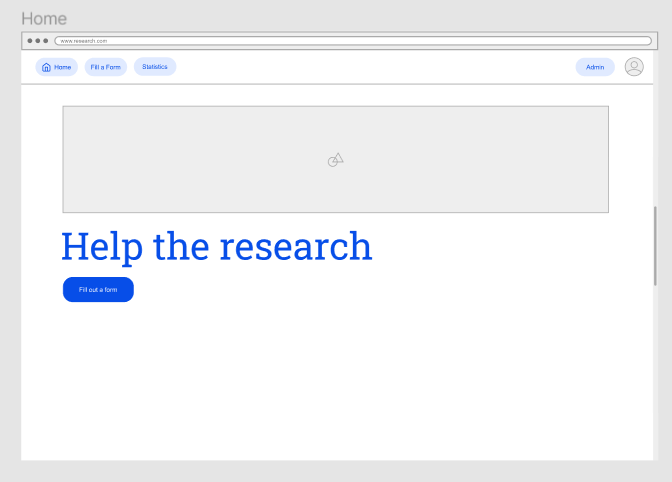
\includegraphics[width=0.8\linewidth]{images/HomeV1.png}
  \captionof{figure}{Home Page}
  \label{fig:HomeV1}
\end{minipage}%
\begin{minipage}{.5\textwidth}
  \centering
  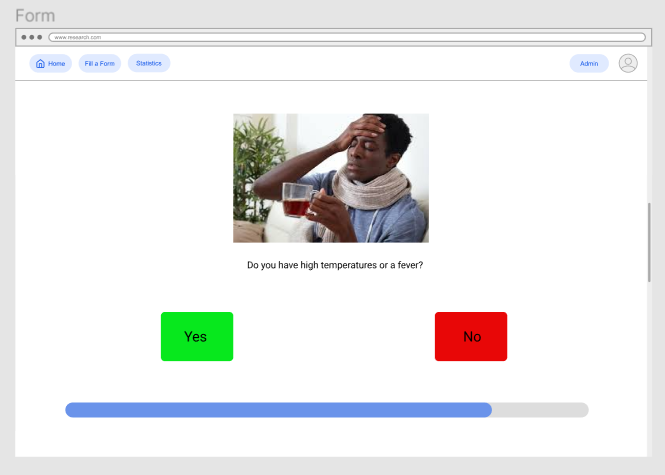
\includegraphics[width=0.8\linewidth]{images/FormV1.png}
  \captionof{figure}{Form Page}
  \label{fig:FormV1}
\end{minipage}
\end{figure}

\begin{figure}[H]
\centering
\begin{minipage}{.5\textwidth}
  \centering
  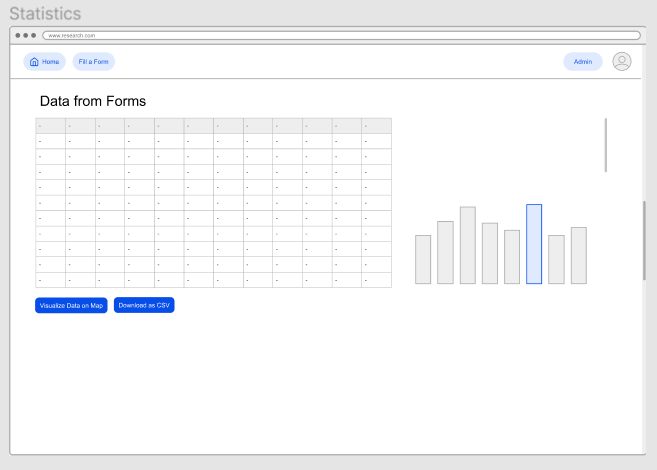
\includegraphics[width=0.8\linewidth]{images/StatsV1.png}
  \captionof{figure}{Stats Page}
  \label{fig:StatsV1}
\end{minipage}%
\begin{minipage}{.5\textwidth}
  \centering
  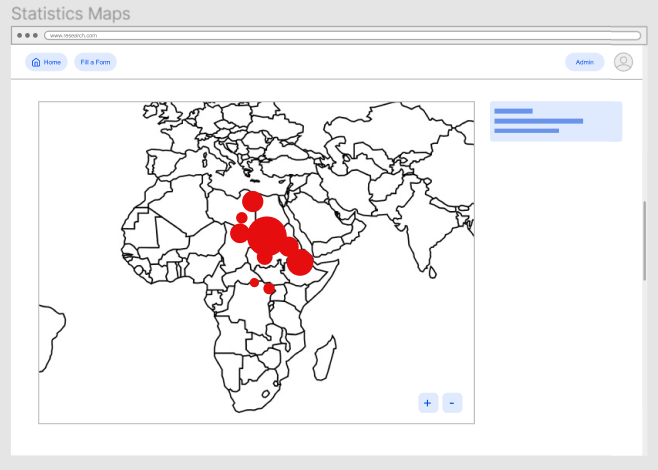
\includegraphics[width=0.8\linewidth]{images/MapV1.png}
  \captionof{figure}{Maps Page}
  \label{fig:MapV1}
\end{minipage}
\end{figure}


%==============================================================================
%% User Personas and Stories

\newpage

\section{User Personas and Stories}
\label{appendix:UPandS}
This is how the site will be used by different groups of users (part of the full user personas):
\begin{itemize}
    \item Public User: have access to public form page.
    \item Medical User: More advanced form page where the data submitted is more trusted.
    \item Professional Users(Vets, Farmers, etc): Also have their own form page with questions specific to their field.
    \item Lower Level Admin (Researchers): Have access to the data and stats pages including maps page which are not public.
    \item Higher Level Admin (Customer): Have access to all the private data and can edit the questionnaires.
\end{itemize}


These are user stories the team made when deciding how each person would view the data collected.

As low level admin:
\begin{itemize}
    \item I want to view data in table so that I can get an overview of what has been reported.
    \item I want to filter this data (by location, symptoms, age etc) so that I can find out more specific information.
    \item I want to have clear information on potential outbreaks so that I can study these areas more closely.
    \item I want a clear web page design so that I can gain an insight into the data at a quick glance.
    \item I want to view data in a mapping format so that I can see potential outbreaks.
    \item I want to be able to access the specific data from a location when clicked on the map so that I can quickly find out what is happening in that area.
\end{itemize}

As high level admin:
\begin{itemize}
    \item I want to view this data to do research on sleeping sickness outbreaks (as above).
    \item I want to be able to delete data that is clearly inaccurate and repeated so it does not distract from genuine data.
    \item I want to be able to review the changes to data (potentially made by professionals) so that I can correct any inaccuracies.
\end{itemize}

(Public and professional users can not view this data and thus don't need stories)

\end{document}
